\documentclass[tikz,border=3pt]{standalone}
\usepackage[T1]{fontenc}
\usepackage{lmodern,amsmath}
\usetikzlibrary{arrows.meta,calc,patterns}
\begin{document}
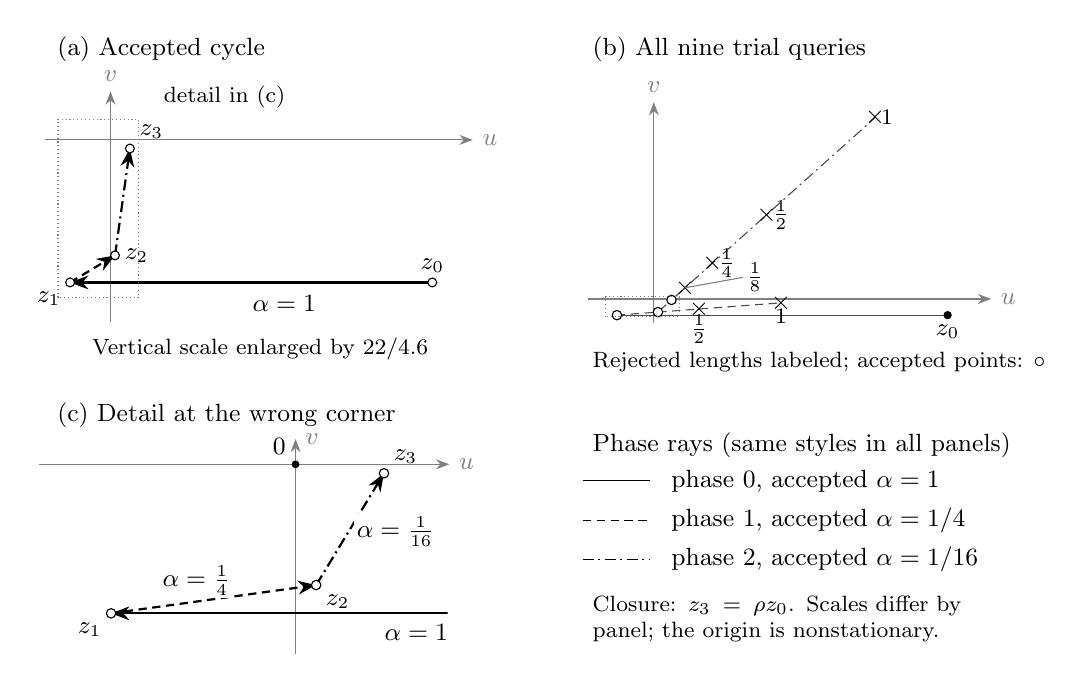
\begin{tikzpicture}[>=Stealth,font=\small,
phase0/.style={solid},phase1/.style={densely dashed},
phase2/.style={dash pattern=on 4pt off 1.6pt on .7pt off 1.6pt}]
\node[anchor=west] at (-.8,1.15) {(a) Accepted cycle};
\begin{scope}[x=4.6cm,y=22cm]
\draw[->,gray] (-.18,0)--(1.0,0) node[right] {$u$};
\draw[->,gray] (0,-.105)--(0,.028) node[above] {$v$};
\draw[->,thick,phase0] (0.888432624,-0.082297398)--(-0.111567376,-0.082297398);
\draw[->,thick,phase1] (-0.111567376,-0.082297398)--(0.012456062,-0.066672398);
\draw[->,thick,phase2] (0.012456062,-0.066672398)--(0.053482939,-0.004954238);
\draw[fill=white] (0.888432624,-0.082297398) circle[radius=1.6pt] node[above] {$z_0$};
\draw[fill=white] (-0.111567376,-0.082297398) circle[radius=1.6pt] node[below left] {$z_1$};
\draw[fill=white] (0.012456062,-0.066672398) circle[radius=1.6pt] node[right] {$z_2$};
\draw[fill=white] (0.053482939,-0.004954238) circle[radius=1.6pt] node[above right] {$z_3$};
\node[below] at (.48,-.084) {$\alpha=1$};
\draw[densely dotted,gray] (-.145,-.091) rectangle (.078,.012);
\node[anchor=west,font=\footnotesize] at (.12,.025) {detail in (c)};
\end{scope}
\node[font=\footnotesize] at (1.9,-2.65) {Vertical scale enlarged by $22/4.6$};
\node[anchor=west] at (6.0,1.15) {(b) All nine trial queries};
\begin{scope}[shift={(6.9cm,-2.02cm)},x=4.2cm,y=2.5cm]
\draw[->,gray] (-.20,0)--(1.02,0) node[right] {$u$};
\draw[->,gray] (0,-.12)--(0,1.0) node[above] {$v$};
\draw[phase0,black!70] (0.888432624,-0.082297398)--(-0.111567376,-0.082297398);
\draw[phase1,black!70] (-0.111567376,-0.082297398)--(0.384526374,-0.019797398);
\draw[phase2,black!70] (0.012456062,-0.066672398)--(0.668886094,0.920818157);
\draw[fill=white] (-0.111567376,-0.082297398) circle[radius=1.7pt];
\node[inner sep=0pt] at (0.384526374,-0.019797398) {$\times$};
\node[below,font=\footnotesize,inner sep=2pt] at (0.384526374,-0.019797398) {$1$};
\node[inner sep=0pt] at (0.136479499,-0.051047398) {$\times$};
\node[below,font=\footnotesize,inner sep=2pt] at (0.136479499,-0.051047398) {$\tfrac{1}{2}$};
\draw[fill=white] (0.012456062,-0.066672398) circle[radius=1.7pt];
\node[inner sep=0pt] at (0.668886094,0.920818157) {$\times$};
\node[right,font=\footnotesize,inner sep=2pt] at (0.668886094,0.920818157) {$1$};
\node[inner sep=0pt] at (0.340671078,0.427072880) {$\times$};
\node[right,font=\footnotesize,inner sep=2pt] at (0.340671078,0.427072880) {$\tfrac{1}{2}$};
\node[inner sep=0pt] at (0.176563570,0.180200241) {$\times$};
\node[right,font=\footnotesize,inner sep=2pt] at (0.176563570,0.180200241) {$\tfrac{1}{4}$};
\node[inner sep=0pt] at (0.094509816,0.056763922) {$\times$};
\draw[gray] (0.094509816,0.056763922)--(.27,.11);\node[right,font=\footnotesize,inner sep=1pt] at (.27,.11) {$\tfrac18$};
\draw[fill=white] (0.053482939,-0.004954238) circle[radius=1.7pt];
\fill (0.888432624,-0.082297398) circle[radius=1.5pt] node[below] {$z_0$};
\draw[densely dotted,gray] (-.145,-.091) rectangle (.078,.012);
\end{scope}
\node[anchor=west,font=\footnotesize] at (6.0,-2.82) {Rejected lengths labeled; accepted points: $\circ$};
\node[anchor=west] at (-.8,-3.50) {(c) Detail at the wrong corner};
\begin{scope}[shift={(2.35cm,-4.12cm)},x=21cm,y=23cm]
\draw[->,gray] (-.155,0)--(.093,0) node[right] {$u$};
\draw[->,gray] (0,-.105)--(0,.014) node[right] {$v$};
\begin{scope}
\clip (-.153,-.10) rectangle (.092,.014);
\draw[->,thick,phase0] (0.888432624,-0.082297398)--(-0.111567376,-0.082297398);
\draw[->,thick,phase1] (-0.111567376,-0.082297398)--(0.012456062,-0.066672398);
\draw[->,thick,phase2] (0.012456062,-0.066672398)--(0.053482939,-0.004954238);
\end{scope}
\draw[fill=white] (-0.111567376,-0.082297398) circle[radius=1.7pt] node[below left] {$z_1$};
\draw[fill=white] (0.012456062,-0.066672398) circle[radius=1.7pt] node[below right] {$z_2$};
\draw[fill=white] (0.053482939,-0.004954238) circle[radius=1.7pt] node[above right] {$z_3$};
\node[above,fill=white,inner sep=1pt] at (-.060,-.074) {$\alpha=\tfrac14$};
\node[right,fill=white,inner sep=1pt] at (.035,-.037) {$\alpha=\tfrac1{16}$};
\node[below] at (.073,-.083) {$\alpha=1$};
\fill (0,0) circle[radius=1.4pt] node[above left] {$0$};
\end{scope}
\begin{scope}[shift={(6.0cm,-3.88cm)}]
\node[anchor=west] at (0,0) {Phase rays (same styles in all panels)};
\draw[phase0] (0,-.45)--(.85,-.45);\node[anchor=west] at (1,-.45) {phase $0$, accepted $\alpha=1$};
\draw[phase1] (0,-.95)--(.85,-.95);\node[anchor=west] at (1,-.95) {phase $1$, accepted $\alpha=1/4$};
\draw[phase2] (0,-1.45)--(.85,-1.45);\node[anchor=west] at (1,-1.45) {phase $2$, accepted $\alpha=1/16$};
\node[anchor=west,font=\footnotesize,align=left,text width=5.2cm] at (0,-2.2) {Closure: $z_3=\rho z_0$. Scales differ by panel; the origin is nonstationary.};
\end{scope}
\end{tikzpicture}
\end{document}
